\author{Марухленко Д.С. @japersik}
\date{\today}

\documentclass[a4paper,12pt]{article}
\usepackage[english,russian]{babel}
\usepackage[utf8]{inputenc}
\usepackage{amsmath,amsfonts,amssymb,amsthm,mathtools}
\usepackage{hyperref}
\usepackage{wrapfig}
\usepackage{array}
\usepackage{tabularx}
\usepackage[left=2.5cm, right=1.5cm, top=2.5cm, bottom=2.5cm]{geometry}

\usepackage{pdfpages}

\usepackage{indentfirst}
\usepackage{stmaryrd}
\usepackage{graphicx}
\setlength\parindent{5ex}

\usepackage{fancyhdr} %%колонтикулы
\usepackage{lastpage}
\pagestyle{fancy}
\fancyhf{}
\rfoot{\thepage}
\cfoot{}
\lfoot{Marukhlenko Daniil 2022}
\renewcommand{\footrulewidth}{0.4pt}

\usepackage{lipsum}
\usepackage{wasysym}
\usepackage{booktabs}
\usepackage{blindtext}
\usepackage{siunitx}


\usepackage{svg}

\newcommand{\authorName}{Марухленко Д.С.}
\newcommand{\workType}{Комплексная лабораторная работа}
\newcommand{\workName}{Устройство для измерения угловых перемещений}
\newcommand{\subjectName}{Преобразователи информации}
\newcommand{\workOption}{}
\newcommand{\groupNumber}{R34352}
\newcommand{\teacherName}{Быстров С.В.}

\begin{document}
    \thispagestyle{empty}
%титульный лист%
\begin{center}
    Национальный исследовательский университет ИТМО\\
    Факультет систем управления и робототехники
    \vskip 7cm

    \Huge \workType                         \\
    \huge <<\workName>>                     \\
    \Large по дисциплине <<\subjectName>>   \\
\end{center}
\vfill

\begin{flushright}
    Подготовили: \authorName         \\
    Группа: \groupNumber            \\
    Преподаватель: \teacherName     \\
\end{flushright}
\vskip 2cm

\begin{center}
    Санкт-Петербург 2022г.
\end{center}
\newpage
    \tableofcontents
    \newpage
    \section{Цель работы}
Ознакомление с устройством бесконтактных датчиков приближения, изучение принципов работы и схем включения.
    \section{Этапы выполнения}
\label{sec:stages}
\begin{table}[!h]
    \centering
    \begin{tabularx}{\textwidth}{
        | >{\raggedright\arraybackslash}>{\hsize=.27\hsize}X
        | >{\centering\arraybackslash}>{\hsize=.45\hsize}X
        | >{\raggedright\arraybackslash}X
        | >{\centering\arraybackslash}>{\hsize=.3\hsize}X
        | >{\centering\arraybackslash}>{\hsize=.9\hsize}X|}
        \hline
        \textbf{Номер этапа} & \textbf{Название этапа} & \textbf{Содержание} & \textbf{Срок исполнения} & \textbf{Дополнительное задание} \\
        \hline \hline
        1 & Патентный поиск & 1. Поиск аналогов по источникам патентной информации (3 аналога разного принципа действия). \newline 2. Сравнительный анализ выбранных аналогов. \newline 3. Выбор принципа действия разрабатываемого устройства. & до 15.10.22 & Поиск двух зарубежных аналогов с включением их в сравнительный анализ \\
        \hline
        2 & Техническое предложение & 1. Библиографический поиск информации о датчиках, выбранного принципа действия (расчетные формулы, схемы включения и т.д.) \newline 2. Разработка функциональной схемы устройства. & до 15.11.22 & Чертеж функциональной схемы \\
        \hline
        3 & Разработка собственного технического решения & 1. Разработка принципиальной электрической схемы (или схемы соединений) вторичного преобразователя (наличие микроконтроллера в схеме – обязательно) \newline 2. Выбор источника(ов) питания. \newline 3. Чертеж Э3 или Э4 & до 30.12.22 & Разработка алгоритма функционирования микроконтроллера \\
        \hline
    \end{tabularx}
    \caption{Этапы выполнения задания}
    \label{tab:stages}
\end{table}
\newpage

    \section{Анализ задания}
\label{sec:analys}

Оптическая скамья -- установка, представляющая из себя массивную направляющую с насаженными на нее рейтерами с оптическими элементами.
Рейтеры можно перемещать и неподвижно закреплять в любом ее месте при сохранении строгой параллельности оптическим и визирным осям.
\begin{figure}[!h]
    \centering
    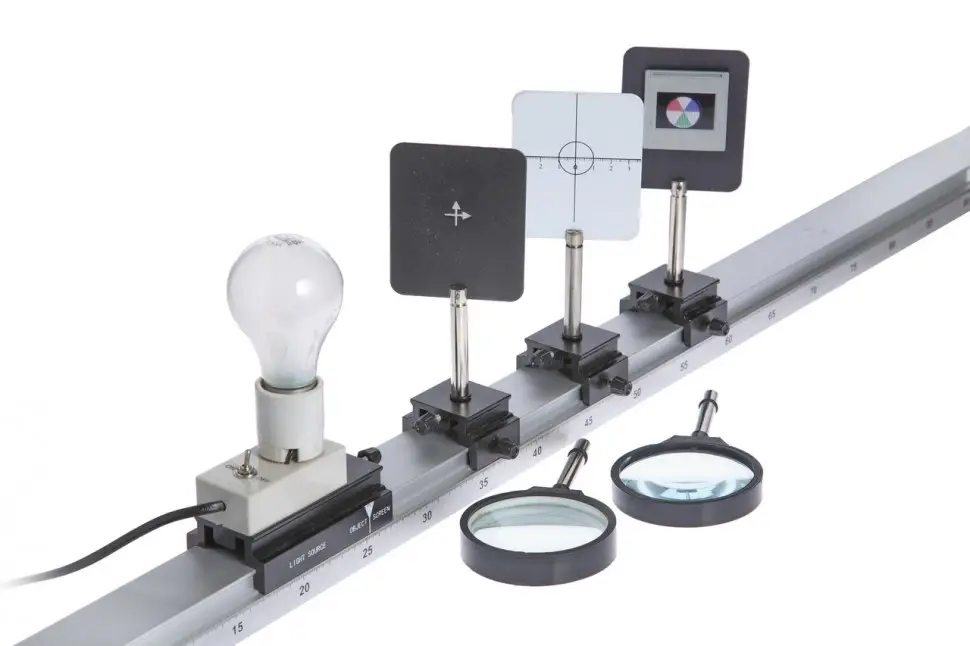
\includegraphics[width=0.5\textwidth]{img/img}
    \caption{Оптическая скамья с рейтерами}
    \label{fig:img}
\end{figure}

Необходимо разработать измерительное устройство для угловых перемещений зеркала относительно его горизонтальной оси.
Устройство должно обладать высокой точностью и относительно небольшим диапазоном измерения ($\pm5^\circ$), что необходимо учитывать при выборе метода измерения.

    \section{Патентный поиск}
\label{sec:patent}
Для поиска аналогов разрабатываемого устройства воспользуемся интернет-ресурсом Федерального института промышленной собственности (\href{https://www1.fips.ru/iiss/db.xhtml}{https://www1.fips.ru/iiss/db.xhtml}) и рассмотрим различные в реализации варианты решения аналогичных задач.
\subsection{Измерение на основе понетциометра}

Принцип работы первого аналога рассматривается в описании изобретения к патенту \textbf{ИЗ №2780031} (Приложение А).

Устройство можно разделить на 3 основные части: источник опорного напряжения, потенциометрический датчик и микроконтроллер для считывания напряжения с датчика.

При измерении используется связь между контролируемым объектом и подвижным контактом потенциометрического датчика.
Датчик закрепляется непосредственно на вращающуюся ось подвижной частью, в неподвижной -- к неподвижной опоре вращающейся оси.
Величина измеряемого напряжения на датчике связана с физическим положением объекта.

Преимуществами такого исполнения измерительного устройства являются:
\begin{itemize}
    \item Относительная простота реализации: датчик представляет из себя переменный делитель напряжения, не требующий сложных вычислений при преобразовании сигнала.
    \item Энергонезависимость датчика: после отключения датчика от источника питания и повторного включения показания не изменяться, в отличие от датчиков, подобных относительным энкодерам.
    \item Компактность измерительного устройства: современный ассортимент потенциометров предлагает весьма широкий выбор устройств с различными параметрами и габаритами.
\end{itemize}

К недостаткам можно отнести:
\begin{itemize}
    \item Необходимость создания источника опорного напряжения.
    \item Стирание резистивного слоя внутри датчика, что ведет к ухудшению точности измерений.
\end{itemize}

\subsection{Измерение на основе магниточувствительного элемента}

Принцип работы второго аналога рассматривается в описании полезной модели к патенту \textbf{ПМ №175216} (Приложение Б).

Полезная модель, описанная в работе, относится к измерительной технике и может быть использована для бесконтактных абсолютных измерений угловых перемещений.
Устройство для измерения угловых перемещений включает подвижный модуль, выполненный в виде вала с винтовой канавкой, образующей на поверхности вала чередующиеся выступы и впадины, сопряженный с объектом пользователя, и магнитный преобразователь, дистанционно взаимодействующий с подвижным модулем, содержащий магниточувствительные элементы, сопряженные с подвижным модулем и плату обработки.

Преимуществами такого исполнения измерительного устройства являются:
\begin{itemize}
    \item Бесконтактный съем показаний: наличие датчика не влияет на свободу перемещения подвижного объекта.
            Так же отсутствие физического контакта повышает износостойкость измерительного прибора.
    \item Малые габариты: современные магниточувствительные элементы имеют малые габариты, не теряя при этом точности измерений.
\end{itemize}

К недостаткам можно отнести:
\begin{itemize}
    \item Необходимость установки резьбового вала на ось вращения зеркала.
    \item Необходимость использования как минимум двух чувствительных элементов для определения направления вращения.
    \item Необходимость установки концевика для калибровки или ручной калибровки положения после каждого отключения от питания.
\end{itemize}

\subsection{Измерение на основе кодового лимба}
Принцип работы третьего аналога рассматривается в описании изобретения к патенту \textbf{ИЗ №2120105} (Приложение В).

Преобразователь угловых перемещений содержит подвижную систему, состоящую из жестко закрепленного на валу кодового лимба, и систему считывания информации, состоящую из последовательно расположенных источников излучения, конденсора и фотоприемного устройства.
Преобразователь содержит также электронный блок в виде блока аналого-цифровой обработки и управления, вход которого связан с выходами фотоприемного устройства.
На кодовый лимб преобразователя наносится одна кодовая дорожка со штрихами.

Преимущества данного способа:
\begin{itemize}
    \item Бесконтактный съем показаний
    \item Энергонезависимость датчика при нанесении уникальной кодировки
\end{itemize}

Недостатки:
\begin{itemize}
    \item Дискретность сигнала, шаг дискретности зависит от физических способностей фотоприемного устройства и возможности точного изготовления кодового лимба.
    \item Необходимость точного исполнения кодового лимба. Небольшие отклонения могут сильно сказаться на точности датчика.
\end{itemize}

\subsection{Выбор принципа действия разрабатываемого устройства}\label{subsec:choise1}

Опираясь на анализ преимуществ и недостатков каждого из способов, было принято решение проводить дальнейшую разработку, опираясь на способ с использованием \underline{потенциометрического} датчика.

Следующие этапы разработки будут включать поиск информации о потенциометрических датчиках, разработку функциональной схемы устройства, разработку принципиальной электрической схемы и выбор источников питания.
Проведенный поиск аналогов будет служить одним из источников информации при их выполнении.

    \section{Техническое предложение}
\subsection{Поиск информации о датчиках выбранного типа действия}

Потенциометрический датчик представляет собой переменный резистор, к которому приложено напряжение.
Выходная величина - разность потенциалов между подвижным контактом и одним из выходов резистора.
Она изменяется в зависимости от линейного или углового перемещения подвижного контакта.

\begin{figure}[!h]
    \centering
    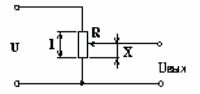
\includegraphics[width=0.5\textwidth]{img/img_1}
    \caption{Электрическая принципиальная схема потенциометрического датчика}
    \label{fig:img_1}
\end{figure}

Потенциометрические датчики по способу выполнения сопротивления делятся на три вида:
\begin{itemize}

    \item Ламельные.

    Используются для проведения относительно грубых измерений.
    Представляют из себя набор постоянных резисторов, подобранных по номиналу и припаянных к ламелям.
    Подвижный токосъемный контакт переключается между выходами резисторов, тем самым ступенчато изменяя параметры делителя напряжения.

    \begin{figure}[!h]
        \centering
        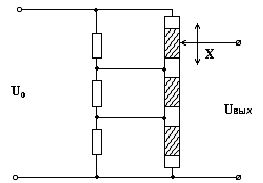
\includegraphics[width=0.5\textwidth]{img/img_2}
        \caption{Ламельный потенциометрический датчик}
        \label{fig:img_2}
    \end{figure}

    Такой тип датчика не подходит для разрабатываемого устройства ввиду низкой точности измерения.

    \item Проволочные с непрерывной намоткой.

    Датчики предназначены для более точных измерений, нежели предыдущий вариант.
    Обычно конструкционно состоят из диэлектрического материала (текстолита, гетинакса, керамики), на который в один слой намотана токопроводящая проволока с высоким удельным сопротивлением (вольфрам, манганин, фехраль).
    Токосъемый контакт, выполненный из более мягкого металла, скользит по зачищенной поверхности проволоки, намотанной на каркас, чем (аналогично предыдущему случаю) изменяет параметры делителя напряжения.

    Класс точности таких датчиком зависит от толщины проволоки и качества исполнения токосъемного контакта.
    \item С резистивным слоем.

    В датчиках с резистивным слоем вместо проволоки, намотанной на каркас, используется плоская пластина с нанесенным на нее резистивным слоем.
    Проводящий слой наносится напылением или химическим способом.
    Подвижный контакт, так же как в проволочном переменном резисторе, передвигается вдоль пластины.

    В отличие от проволочных потенциометров, точность потенциометров с резистивным слоем не зависит от диаметра используемой проволоки ввиду ее отсутствия.
    Здесь точность определяется точность нанесения резистивного слоя и качеством изготовления подвижного контакта.

\end{itemize}

С учетом описанных преимуществ и недостатков в разрабатываемом устройстве решено использовать потенциометр с резистивным слоем.
Такое исполнение является наиболее точным, а так же датчики и использованием резистивного слоя наиболее компактны.

\subsection{Разработка функциональной схемы устройства}

\begin{figure}[!h]
    \centering
    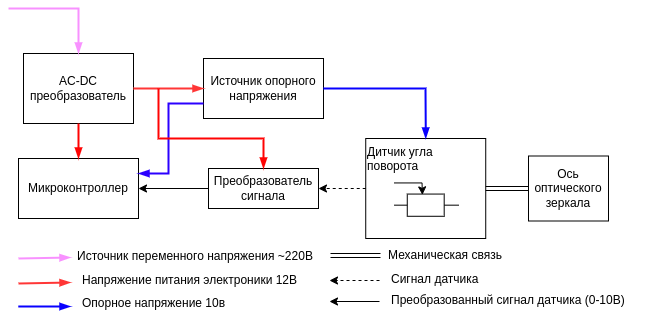
\includegraphics[width=0.9\textwidth]{img/ПИ.drawio}
    \caption{Функциональная схема измерительного устройства и его подключения к микроконтроллеру}
    \label{fig:drawio}
\end{figure}

Система питания устройства состоит из:
\begin{itemize}
    \item Источника переменного тока напряжением 220В;
    \item AC-DC преобразователя (источника постоянного напряжения 12В);
    \item Источника опорного напряжения 10В, в качестве которого может использоваться линейный стабилизатор напряжения;
    \item Используется для устранения погрешностей измерения, связанных с пульсациями в источнике питания.
\end{itemize}

Система измерения состоит из
\begin{itemize}
    \item Потенциометрического датчика углового положения, жестко связанного механически с осью зеркала(см задание);
    \item Преобразователя сигнала, масштабирующего и перемещающего выходной сигнал в требуемый диапазон (0-10В).
    Реализация планируется с использованием операционного усилителя и будет описано в следующей части.
\end{itemize}
\newpage

    \section{Разработка собственного технического решения}
\label{sec:---}
Как уже было описано ранее, в качестве датчика было решено выбрать потенциометрический датчик угла поворота.
К двум контактам датчика подключается источник опорного напряжения (10В), а на третьем формируется напряжение, величина которого зависит от угла поворота.

Так как измерительное устройство состоит из резистивных элементов большого номинала, в качестве источника опорного напряжения используем параметрический стабилизатор напряжения на стабилитроне.
\begin{figure}[!h]
    \centering
    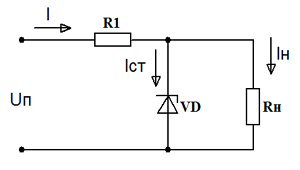
\includegraphics[width=0.5\textwidth]{img/img_4}
    \caption{Схема параметрического стабилизатора напряжения}
    \label{fig:img_4}
\end{figure}

В техническом задании указано, что диапазон измерения должен составлять от $\pm 5 ^\circ$.
Таким образом ширина диапазона измерений составляет $10^\circ$.
Изучение каталогов в поисках датчика с таким диапазоном измерений не привело к положительному результату: потенциометрические датчики угла поворота имеют больший допустимый угол поворота.
В связи с этим, необходимо использовать датчик с бОльшим диапазоном измерений, но использовать его только в требуемом.

\begin{figure}[!h]
    \centering
    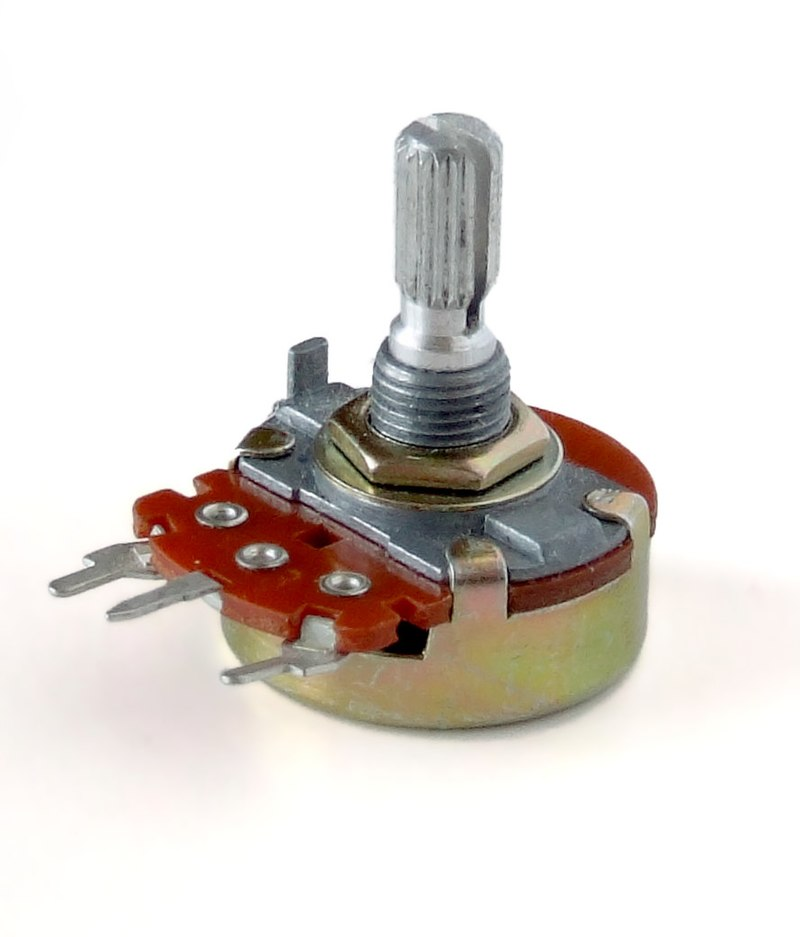
\includegraphics[width=0.4\textwidth]{img/img_3}
    \caption{Потенциометр B10K (WH148)}
    \label{fig:img3}
\end{figure}


Для примера рассмотрим вариант использования потенциометра B10K (WH148).
Его диапазон вращения составляет $300^\circ$.
Установим нулевую точку как поворот на $150^\circ$.
Соответственно, рабочим диапазоном потенциометра будет диапазон от $145^\circ$до $155^\circ$.
Минимальное и максимальное значение выходного напряжения потенциометра будет составлять:
\begin{gather*}
    U_{rout_{min}} = \frac{10\cdot145}{300}= 4.833\text{(В)}\\
    U_{rout_{max}} = \frac{10\cdot155}{300}= 5.167\text{(В)}
\end{gather*}
%https://chipenable.ru/index.php/how-connection/157-masshtabirovanie-signala-operacionnim-usilitelem.html

Это не соответствует заявленным требованиям.
Для решения возникшей проблемы воспользуемся масштабирующей схемой с операционным усилителем.

Выходное напряжение такой схемы считается по формуле:
\begin{gather*}
    U_{aout} = U_{ain}(1 + \frac{R_3}{R_2} + \frac{R_3}{R_1})-V_{cc}\frac{R_3}{R_1}
\end{gather*}

Выберем произвольное $R_3$ из ряда стандартных значений, например, 10кОм и рассчитаем номиналы $R_2$ и $R_1$ из системы уравнений:
\begin{gather*}
    \begin{cases}
        U_{aout_{min}} = U_{ain_{min}}(1 + \frac{R_3}{R_2} + \frac{R_3}{R_1})-V_{cc}\frac{R_3}{R_1}\\
        U_{aout_{max}} = U_{ain_{max}}(1 + \frac{R_3}{R_2} + \frac{R_3}{R_1})-V_{cc}\frac{R_3}{R_1}
    \end{cases}
\end{gather*}
\begin{gather*}
    \begin{cases}
        0 = 4.833(1 + \frac{10^4}{R_2} + \frac{10^4}{R_1})-10\frac{10^4}{R_1}\\
        10 = 5.167(1 + \frac{10^4}{R_2} + \frac{10^4}{R_1})-10\frac{10^4}{R_1}
    \end{cases}
\end{gather*}

\begin{gather*}
        R_1 = 6910.821\text{(Ом)}\ \
        R_2 = 6910.821\text{(Ом)}
\end{gather*}

Найдем ближайшие по номиналу стандартные значения:
\begin{gather*}
    R_1 = 6.8\text{(кОм)}\ \
    R_2 = 6.8\text{(кОм)}
\end{gather*}

Соберем схему измерительного устройства в программе LTspice и проведем моделирование:

\begin{figure}[!h]
    \centering
    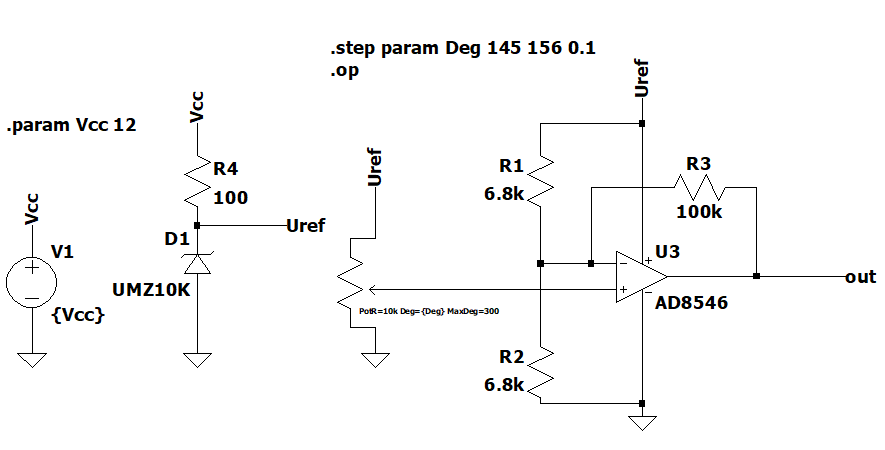
\includegraphics[width=0.7\textwidth]{img/img_5}
    \caption{Схема моделирования измерительного устройства}
    \label{fig:img_5}
\end{figure}
\newpage
\begin{figure}[!h]
    \centering
    \begin{minipage}{0.5\textwidth}
        \centering
        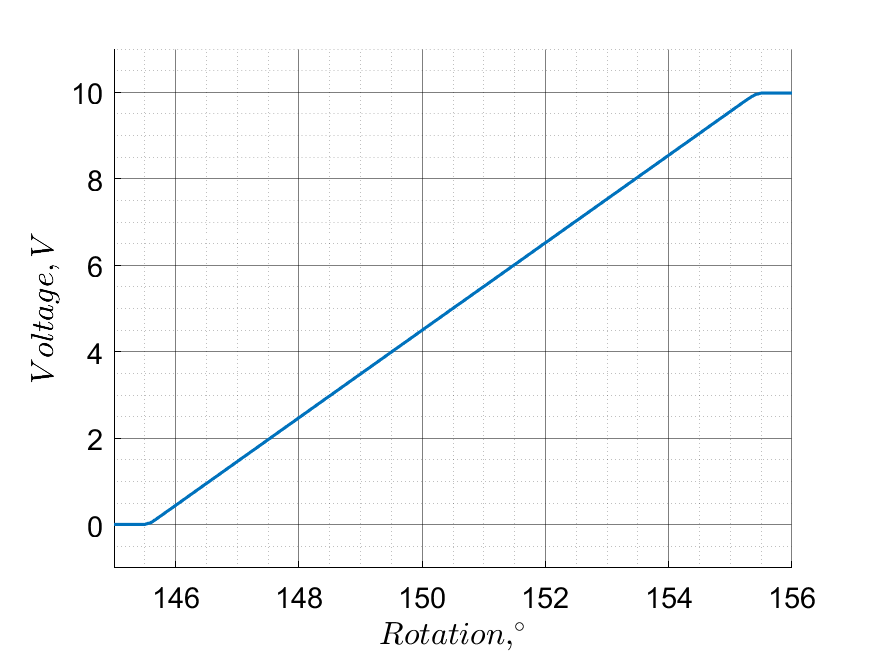
\includegraphics[width = 1\textwidth]{img/img_6}
        Без смещения
        \label{fig:img/img_5}
    \end{minipage}%
\begin{minipage}{0.5\textwidth}
        \centering
        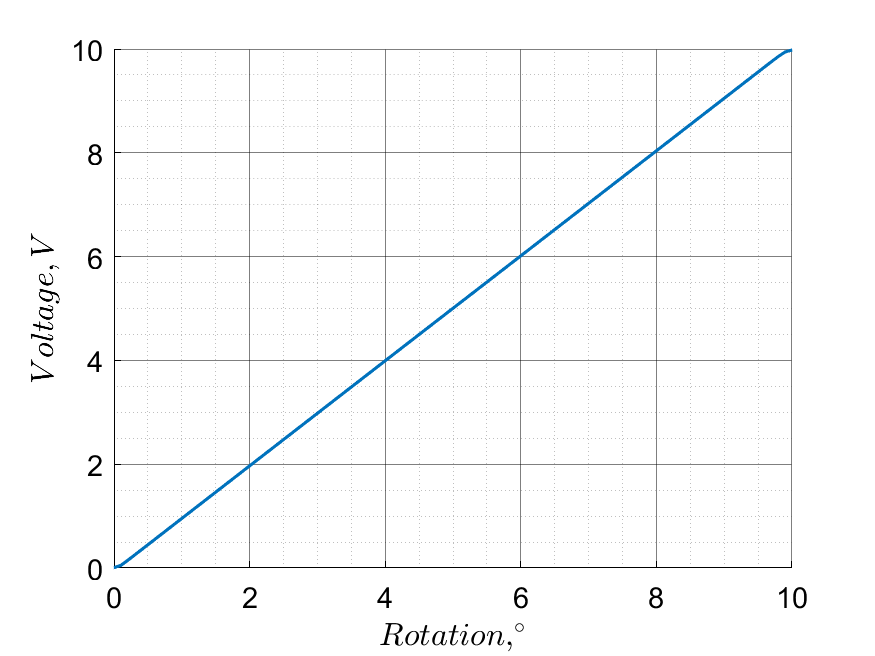
\includegraphics[width = 1\textwidth]{img/img_7}
        Со смещением
        \label{fig:img/img_7}
    \end{minipage}%
    \caption{Зависимость выходного напряжения от угла поворота}
\end{figure}

Как можно заметить, устройство соответствует техническому заданию: в диапазоне измерения $10\circ$ выходной сигнал (напряжение) изменяется в диапазоне 0--10В.

Остается выбрать источник питания: максимальное потребление схемы ограничено резистором $R_4$ (рисунок \ref{fig:img_5}):
\begin{gather*}
    P_{max} = U_{in}I_{max}\\
    I_{max} = \frac{U_{in}}{R_4}\\
    P_{max} = \frac{U^2_{in}}{R_4} = \frac{12^2}{100} = \frac{144}{100}=1.44(\text{Вт})
\end{gather*}
В связи с этим в качестве источника питания может быть выбран практически любой блок питания с ранее описанным напряжением 12В.
Например EPS-15-12 -- AC-DC блок питания со входным напряжением 85В -- 264В переменного тока и выходными 12В 1.25А постоянного (15Вт, что больше требуемого).
\begin{figure}[!h]
    \centering
    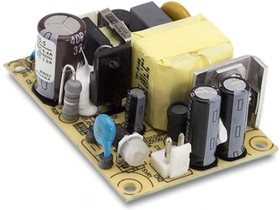
\includegraphics[width=0.5\textwidth]{img/img_8}
    \caption{Блок питания EPS-15-12}
    \label{fig:img_8}
\end{figure}

Выходной контакт измерительного устройства подключается к программируемому логическому контроллеру или микроконтроллеру, имеющему аналоговый вход с 10-вольтовым аналогово-цифровым преобразователем.
\newpage
    \newpage
\section{Приложение A. Устройство для измерения угла положения и линейного перемещения контролируемого объекта ИЗ №2780031}\label{sec:applicationA}
\begin{figure}[!h]
    \centering
    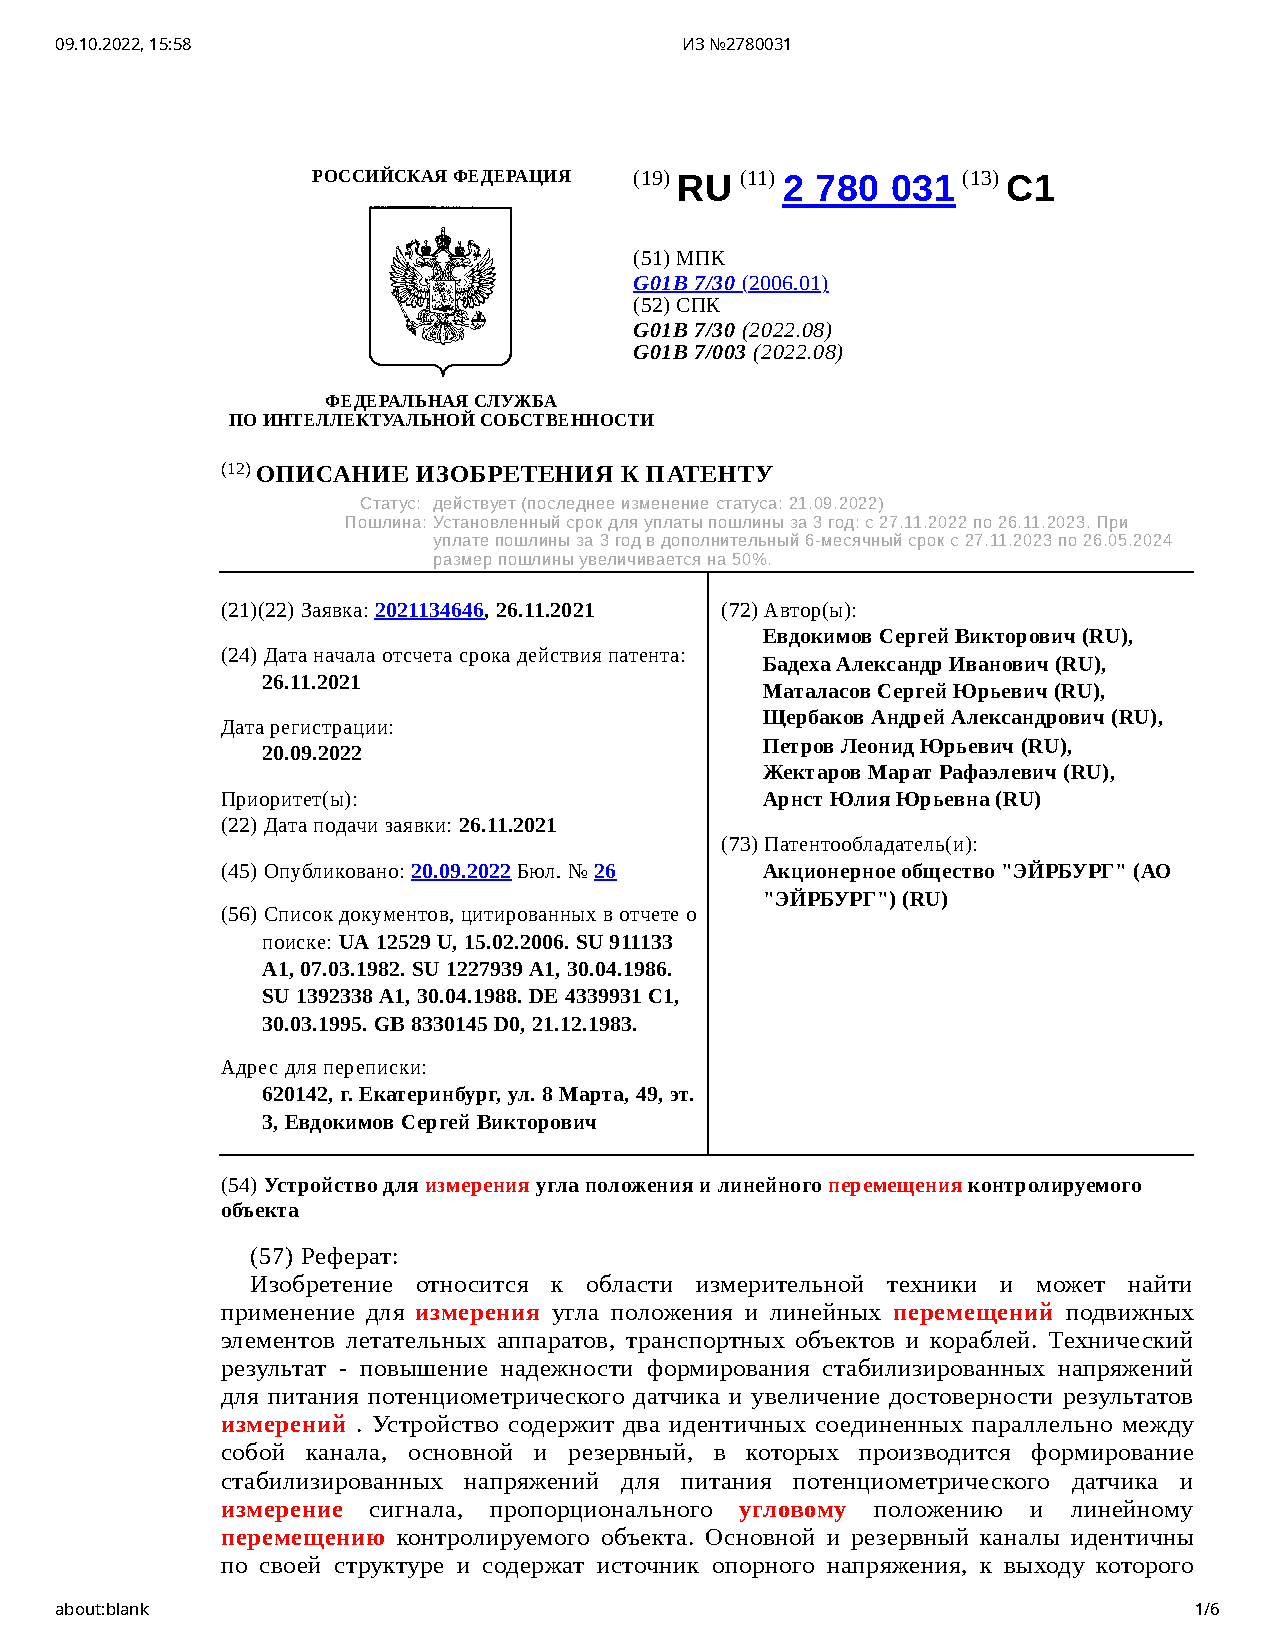
\includepdf[pages=1,width=1.1\textwidth]{pdf/2.pdf}
    \label{fig:app2.1}
\end{figure}
\newpage
\begin{figure}[!h]
    \centering
    \includepdf[pages=2,width=1.1\textwidth]{pdf/2.pdf}
    \label{fig:app2.2}
\end{figure}
\newpage

\begin{figure}[!h]
    \centering
    \includepdf[pages=3,width=1.1\textwidth]{pdf/2.pdf}
    \label{fig:app2.3}
\end{figure}
\newpage

\begin{figure}[!h]
    \centering
    \includepdf[pages=4,width=1.1\textwidth]{pdf/2.pdf}
    \label{fig:app2.4}
\end{figure}
\newpage

\begin{figure}[!h]
    \centering
    \includepdf[pages=5,width=1.1\textwidth]{pdf/2.pdf}
    \label{fig:app2.5}
\end{figure}
\newpage

\begin{figure}[!h]
    \centering
    \includepdf[pages=6,width=1.1\textwidth]{pdf/2.pdf}
    \label{fig:app2.6}
\end{figure}
\newpage

\section{Приложение Б. Преобразователь угловых перемещений ПМ №175216}\label{sec:applicationB}

\begin{figure}[!h]
    \centering
    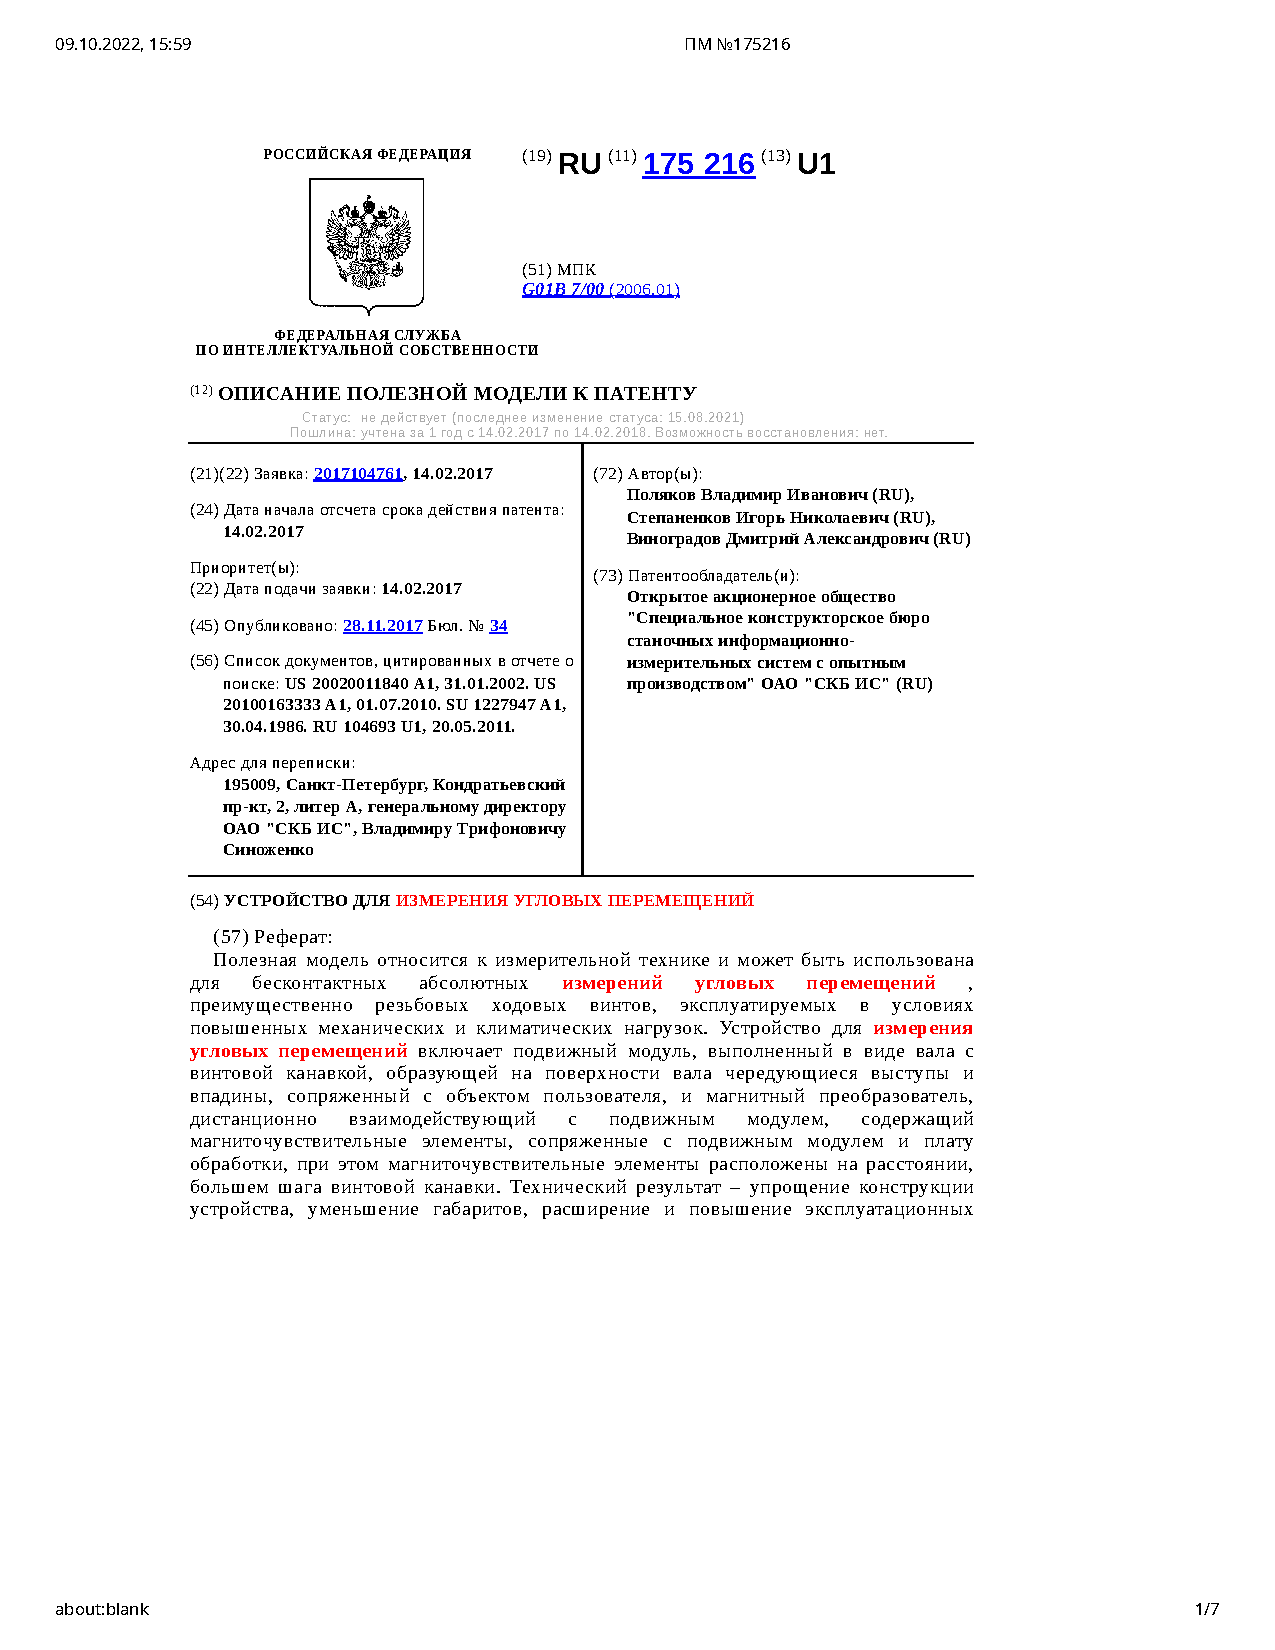
\includepdf[pages=1,width=1.1\textwidth]{pdf/3.pdf}
    \label{fig:app3.1}
\end{figure}
\newpage
\begin{figure}[!h]
    \centering
    \includepdf[pages=2,width=1.1\textwidth]{pdf/3.pdf}
    \label{fig:app3.2}
\end{figure}
\newpage

\begin{figure}[!h]
    \centering
    \includepdf[pages=3,width=1.1\textwidth]{pdf/3.pdf}
    \label{fig:app3.3}
\end{figure}
\newpage

\begin{figure}[!h]
    \centering
    \includepdf[pages=4,width=1.1\textwidth]{pdf/3.pdf}
    \label{fig:app3.4}
\end{figure}
\newpage

\begin{figure}[!h]
    \centering
    \includepdf[pages=5,width=1.1\textwidth]{pdf/3.pdf}
    \label{fig:app3.5}
\end{figure}
\newpage

\begin{figure}[!h]
    \centering
    \includepdf[pages=6,width=1.1\textwidth]{pdf/3.pdf}
    \label{fig:app3.6}
\end{figure}
\newpage

\begin{figure}[!h]
    \centering
    \includepdf[pages=7,width=1.1\textwidth]{pdf/3.pdf}
    \label{fig:app3.7}
\end{figure}
\newpage
\section{Приложение В. Преобразователь угловых перемещений ИЗ №2120105}\label{sec:applicationW}
\begin{figure}[!h]
    \centering
    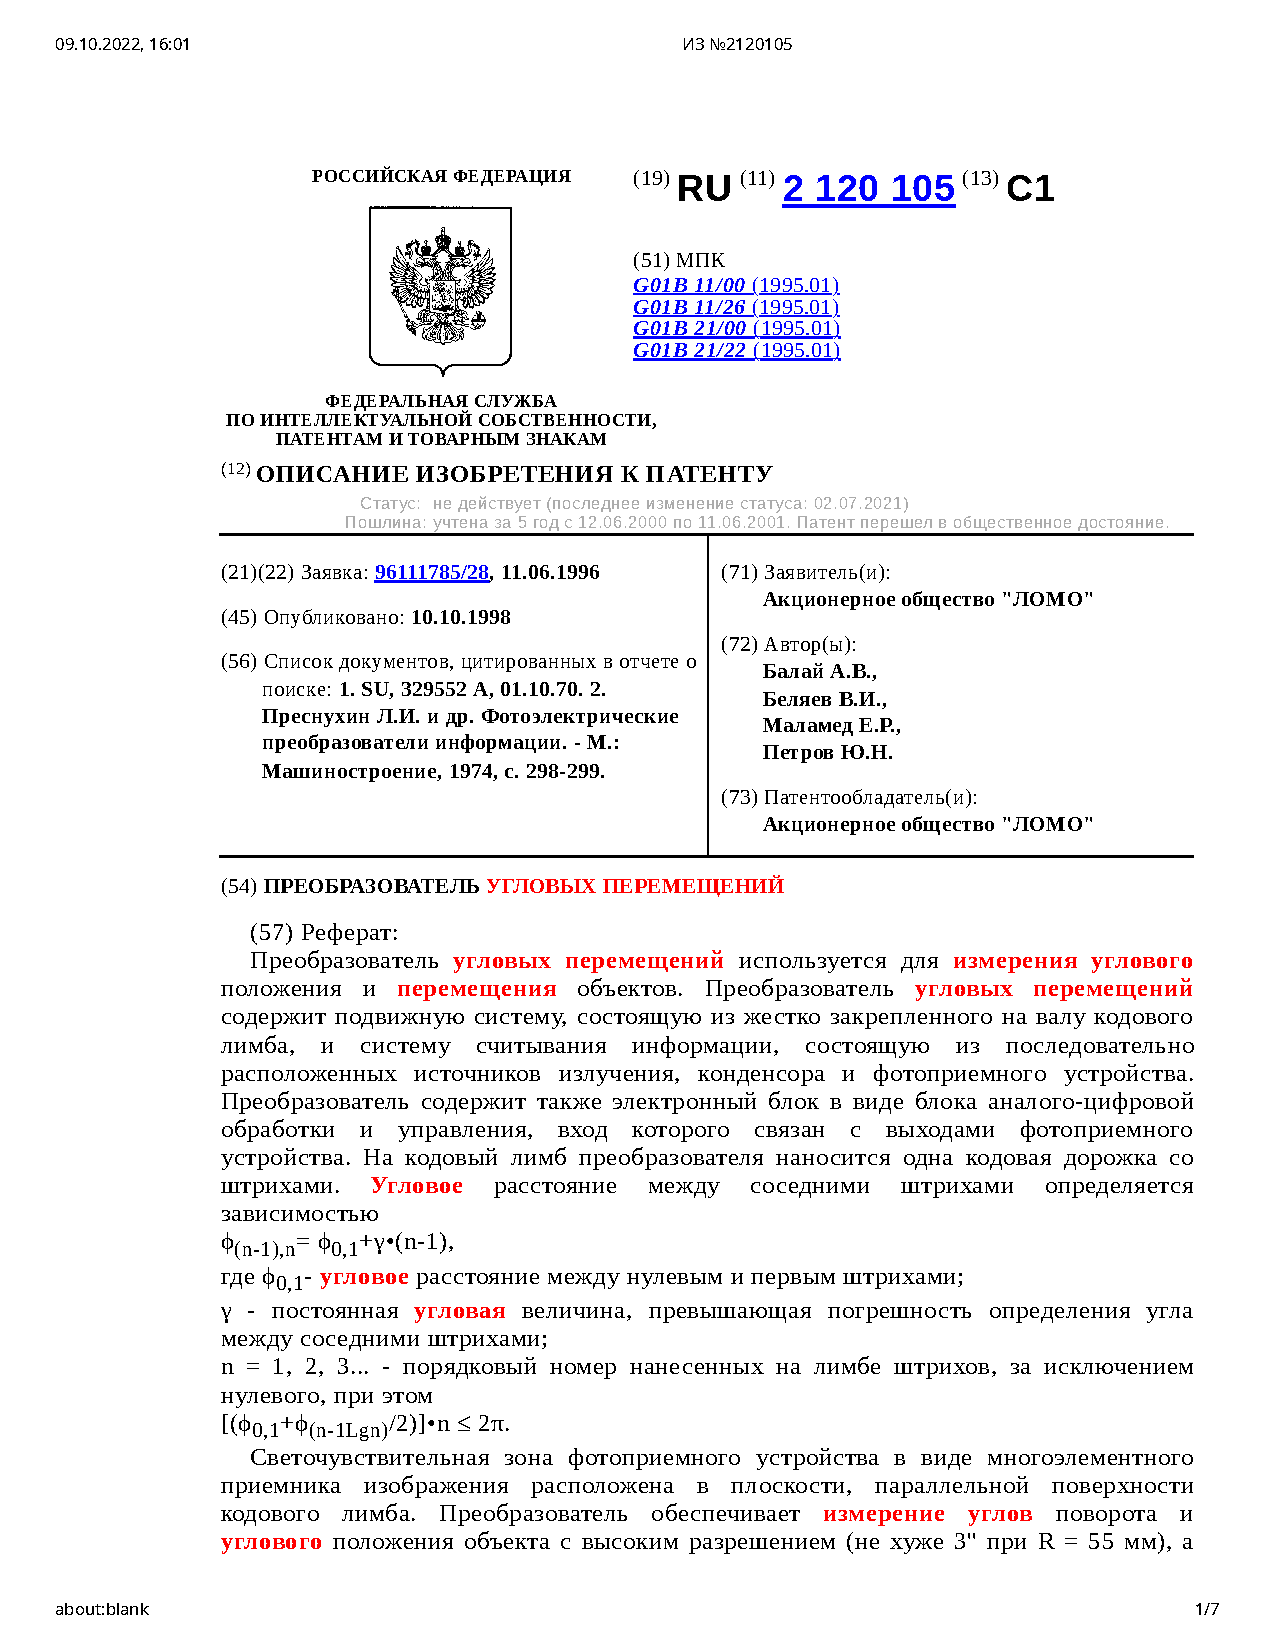
\includepdf[pages=1,width=1.1\textwidth]{pdf/1.pdf}
    \label{fig:app1.1}
\end{figure}
\newpage
\begin{figure}[!h]
    \centering
    \includepdf[pages=2,width=1.1\textwidth]{pdf/1.pdf}
    \label{fig:app1.2}
\end{figure}
\newpage

\begin{figure}[!h]
    \centering
    \includepdf[pages=3,width=1.1\textwidth]{pdf/1.pdf}
    \label{fig:app1.3}
\end{figure}
\newpage

\begin{figure}[!h]
    \centering
    \includepdf[pages=4,width=1.1\textwidth]{pdf/1.pdf}
    \label{fig:app1.4}
\end{figure}
\newpage

\begin{figure}[!h]
    \centering
    \includepdf[pages=5,width=1.1\textwidth]{pdf/1.pdf}
    \label{fig:app1.5}
\end{figure}
\newpage

\begin{figure}[!h]
    \centering
    \includepdf[pages=6,width=1.1\textwidth]{pdf/1.pdf}
    \label{fig:app1.6}
\end{figure}
\newpage

\begin{figure}[!h]
    \centering
    \includepdf[pages=7,width=1.1\textwidth]{pdf/1.pdf}
    \label{fig:app1.7}
\end{figure}


\end{document}